% Options for packages loaded elsewhere
\PassOptionsToPackage{unicode}{hyperref}
\PassOptionsToPackage{hyphens}{url}
%
\documentclass[
]{article}
\usepackage{amsmath,amssymb}
\usepackage{lmodern}
\usepackage{ifxetex,ifluatex}
\ifnum 0\ifxetex 1\fi\ifluatex 1\fi=0 % if pdftex
  \usepackage[T1]{fontenc}
  \usepackage[utf8]{inputenc}
  \usepackage{textcomp} % provide euro and other symbols
\else % if luatex or xetex
  \usepackage{unicode-math}
  \defaultfontfeatures{Scale=MatchLowercase}
  \defaultfontfeatures[\rmfamily]{Ligatures=TeX,Scale=1}
\fi
% Use upquote if available, for straight quotes in verbatim environments
\IfFileExists{upquote.sty}{\usepackage{upquote}}{}
\IfFileExists{microtype.sty}{% use microtype if available
  \usepackage[]{microtype}
  \UseMicrotypeSet[protrusion]{basicmath} % disable protrusion for tt fonts
}{}
\makeatletter
\@ifundefined{KOMAClassName}{% if non-KOMA class
  \IfFileExists{parskip.sty}{%
    \usepackage{parskip}
  }{% else
    \setlength{\parindent}{0pt}
    \setlength{\parskip}{6pt plus 2pt minus 1pt}}
}{% if KOMA class
  \KOMAoptions{parskip=half}}
\makeatother
\usepackage{xcolor}
\IfFileExists{xurl.sty}{\usepackage{xurl}}{} % add URL line breaks if available
\IfFileExists{bookmark.sty}{\usepackage{bookmark}}{\usepackage{hyperref}}
\hypersetup{
  hidelinks,
  pdfcreator={LaTeX via pandoc}}
\urlstyle{same} % disable monospaced font for URLs
\usepackage[margin=1in]{geometry}
\usepackage{color}
\usepackage{fancyvrb}
\newcommand{\VerbBar}{|}
\newcommand{\VERB}{\Verb[commandchars=\\\{\}]}
\DefineVerbatimEnvironment{Highlighting}{Verbatim}{commandchars=\\\{\}}
% Add ',fontsize=\small' for more characters per line
\usepackage{framed}
\definecolor{shadecolor}{RGB}{248,248,248}
\newenvironment{Shaded}{\begin{snugshade}}{\end{snugshade}}
\newcommand{\AlertTok}[1]{\textcolor[rgb]{0.94,0.16,0.16}{#1}}
\newcommand{\AnnotationTok}[1]{\textcolor[rgb]{0.56,0.35,0.01}{\textbf{\textit{#1}}}}
\newcommand{\AttributeTok}[1]{\textcolor[rgb]{0.77,0.63,0.00}{#1}}
\newcommand{\BaseNTok}[1]{\textcolor[rgb]{0.00,0.00,0.81}{#1}}
\newcommand{\BuiltInTok}[1]{#1}
\newcommand{\CharTok}[1]{\textcolor[rgb]{0.31,0.60,0.02}{#1}}
\newcommand{\CommentTok}[1]{\textcolor[rgb]{0.56,0.35,0.01}{\textit{#1}}}
\newcommand{\CommentVarTok}[1]{\textcolor[rgb]{0.56,0.35,0.01}{\textbf{\textit{#1}}}}
\newcommand{\ConstantTok}[1]{\textcolor[rgb]{0.00,0.00,0.00}{#1}}
\newcommand{\ControlFlowTok}[1]{\textcolor[rgb]{0.13,0.29,0.53}{\textbf{#1}}}
\newcommand{\DataTypeTok}[1]{\textcolor[rgb]{0.13,0.29,0.53}{#1}}
\newcommand{\DecValTok}[1]{\textcolor[rgb]{0.00,0.00,0.81}{#1}}
\newcommand{\DocumentationTok}[1]{\textcolor[rgb]{0.56,0.35,0.01}{\textbf{\textit{#1}}}}
\newcommand{\ErrorTok}[1]{\textcolor[rgb]{0.64,0.00,0.00}{\textbf{#1}}}
\newcommand{\ExtensionTok}[1]{#1}
\newcommand{\FloatTok}[1]{\textcolor[rgb]{0.00,0.00,0.81}{#1}}
\newcommand{\FunctionTok}[1]{\textcolor[rgb]{0.00,0.00,0.00}{#1}}
\newcommand{\ImportTok}[1]{#1}
\newcommand{\InformationTok}[1]{\textcolor[rgb]{0.56,0.35,0.01}{\textbf{\textit{#1}}}}
\newcommand{\KeywordTok}[1]{\textcolor[rgb]{0.13,0.29,0.53}{\textbf{#1}}}
\newcommand{\NormalTok}[1]{#1}
\newcommand{\OperatorTok}[1]{\textcolor[rgb]{0.81,0.36,0.00}{\textbf{#1}}}
\newcommand{\OtherTok}[1]{\textcolor[rgb]{0.56,0.35,0.01}{#1}}
\newcommand{\PreprocessorTok}[1]{\textcolor[rgb]{0.56,0.35,0.01}{\textit{#1}}}
\newcommand{\RegionMarkerTok}[1]{#1}
\newcommand{\SpecialCharTok}[1]{\textcolor[rgb]{0.00,0.00,0.00}{#1}}
\newcommand{\SpecialStringTok}[1]{\textcolor[rgb]{0.31,0.60,0.02}{#1}}
\newcommand{\StringTok}[1]{\textcolor[rgb]{0.31,0.60,0.02}{#1}}
\newcommand{\VariableTok}[1]{\textcolor[rgb]{0.00,0.00,0.00}{#1}}
\newcommand{\VerbatimStringTok}[1]{\textcolor[rgb]{0.31,0.60,0.02}{#1}}
\newcommand{\WarningTok}[1]{\textcolor[rgb]{0.56,0.35,0.01}{\textbf{\textit{#1}}}}
\usepackage{graphicx}
\makeatletter
\def\maxwidth{\ifdim\Gin@nat@width>\linewidth\linewidth\else\Gin@nat@width\fi}
\def\maxheight{\ifdim\Gin@nat@height>\textheight\textheight\else\Gin@nat@height\fi}
\makeatother
% Scale images if necessary, so that they will not overflow the page
% margins by default, and it is still possible to overwrite the defaults
% using explicit options in \includegraphics[width, height, ...]{}
\setkeys{Gin}{width=\maxwidth,height=\maxheight,keepaspectratio}
% Set default figure placement to htbp
\makeatletter
\def\fps@figure{htbp}
\makeatother
\setlength{\emergencystretch}{3em} % prevent overfull lines
\providecommand{\tightlist}{%
  \setlength{\itemsep}{0pt}\setlength{\parskip}{0pt}}
\setcounter{secnumdepth}{-\maxdimen} % remove section numbering
<!--radix_placeholder_navigation_in_header-->
<meta name="distill:offset" content=""/>

<script type="application/javascript">

  window.headroom_prevent_pin = false;

  window.document.addEventListener("DOMContentLoaded", function (event) {

    // initialize headroom for banner
    var header = $('header').get(0);
    var headerHeight = header.offsetHeight;
    var headroom = new Headroom(header, {
      tolerance: 5,
      onPin : function() {
        if (window.headroom_prevent_pin) {
          window.headroom_prevent_pin = false;
          headroom.unpin();
        }
      }
    });
    headroom.init();
    if(window.location.hash)
      headroom.unpin();
    $(header).addClass('headroom--transition');

    // offset scroll location for banner on hash change
    // (see: https://github.com/WickyNilliams/headroom.js/issues/38)
    window.addEventListener("hashchange", function(event) {
      window.scrollTo(0, window.pageYOffset - (headerHeight + 25));
    });

    // responsive menu
    $('.distill-site-header').each(function(i, val) {
      var topnav = $(this);
      var toggle = topnav.find('.nav-toggle');
      toggle.on('click', function() {
        topnav.toggleClass('responsive');
      });
    });

    // nav dropdowns
    $('.nav-dropbtn').click(function(e) {
      $(this).next('.nav-dropdown-content').toggleClass('nav-dropdown-active');
      $(this).parent().siblings('.nav-dropdown')
         .children('.nav-dropdown-content').removeClass('nav-dropdown-active');
    });
    $("body").click(function(e){
      $('.nav-dropdown-content').removeClass('nav-dropdown-active');
    });
    $(".nav-dropdown").click(function(e){
      e.stopPropagation();
    });
  });
</script>

<style type="text/css">

/* Theme (user-documented overrideables for nav appearance) */

.distill-site-nav {
  color: rgba(255, 255, 255, 0.8);
  background-color: #0F2E3D;
  font-size: 15px;
  font-weight: 300;
}

.distill-site-nav a {
  color: inherit;
  text-decoration: none;
}

.distill-site-nav a:hover {
  color: white;
}

@media print {
  .distill-site-nav {
    display: none;
  }
}

.distill-site-header {

}

.distill-site-footer {

}


/* Site Header */

.distill-site-header {
  width: 100%;
  box-sizing: border-box;
  z-index: 3;
}

.distill-site-header .nav-left {
  display: inline-block;
  margin-left: 8px;
}

@media screen and (max-width: 768px) {
  .distill-site-header .nav-left {
    margin-left: 0;
  }
}


.distill-site-header .nav-right {
  float: right;
  margin-right: 8px;
}

.distill-site-header a,
.distill-site-header .title {
  display: inline-block;
  text-align: center;
  padding: 14px 10px 14px 10px;
}

.distill-site-header .title {
  font-size: 18px;
  min-width: 150px;
}

.distill-site-header .logo {
  padding: 0;
}

.distill-site-header .logo img {
  display: none;
  max-height: 20px;
  width: auto;
  margin-bottom: -4px;
}

.distill-site-header .nav-image img {
  max-height: 18px;
  width: auto;
  display: inline-block;
  margin-bottom: -3px;
}



@media screen and (min-width: 1000px) {
  .distill-site-header .logo img {
    display: inline-block;
  }
  .distill-site-header .nav-left {
    margin-left: 20px;
  }
  .distill-site-header .nav-right {
    margin-right: 20px;
  }
  .distill-site-header .title {
    padding-left: 12px;
  }
}


.distill-site-header .nav-toggle {
  display: none;
}

.nav-dropdown {
  display: inline-block;
  position: relative;
}

.nav-dropdown .nav-dropbtn {
  border: none;
  outline: none;
  color: rgba(255, 255, 255, 0.8);
  padding: 16px 10px;
  background-color: transparent;
  font-family: inherit;
  font-size: inherit;
  font-weight: inherit;
  margin: 0;
  margin-top: 1px;
  z-index: 2;
}

.nav-dropdown-content {
  display: none;
  position: absolute;
  background-color: white;
  min-width: 200px;
  border: 1px solid rgba(0,0,0,0.15);
  border-radius: 4px;
  box-shadow: 0px 8px 16px 0px rgba(0,0,0,0.1);
  z-index: 1;
  margin-top: 2px;
  white-space: nowrap;
  padding-top: 4px;
  padding-bottom: 4px;
}

.nav-dropdown-content hr {
  margin-top: 4px;
  margin-bottom: 4px;
  border: none;
  border-bottom: 1px solid rgba(0, 0, 0, 0.1);
}

.nav-dropdown-active {
  display: block;
}

.nav-dropdown-content a, .nav-dropdown-content .nav-dropdown-header {
  color: black;
  padding: 6px 24px;
  text-decoration: none;
  display: block;
  text-align: left;
}

.nav-dropdown-content .nav-dropdown-header {
  display: block;
  padding: 5px 24px;
  padding-bottom: 0;
  text-transform: uppercase;
  font-size: 14px;
  color: #999999;
  white-space: nowrap;
}

.nav-dropdown:hover .nav-dropbtn {
  color: white;
}

.nav-dropdown-content a:hover {
  background-color: #ddd;
  color: black;
}

.nav-right .nav-dropdown-content {
  margin-left: -45%;
  right: 0;
}

@media screen and (max-width: 768px) {
  .distill-site-header a, .distill-site-header .nav-dropdown  {display: none;}
  .distill-site-header a.nav-toggle {
    float: right;
    display: block;
  }
  .distill-site-header .title {
    margin-left: 0;
  }
  .distill-site-header .nav-right {
    margin-right: 0;
  }
  .distill-site-header {
    overflow: hidden;
  }
  .nav-right .nav-dropdown-content {
    margin-left: 0;
  }
}


@media screen and (max-width: 768px) {
  .distill-site-header.responsive {position: relative; min-height: 500px; }
  .distill-site-header.responsive a.nav-toggle {
    position: absolute;
    right: 0;
    top: 0;
  }
  .distill-site-header.responsive a,
  .distill-site-header.responsive .nav-dropdown {
    display: block;
    text-align: left;
  }
  .distill-site-header.responsive .nav-left,
  .distill-site-header.responsive .nav-right {
    width: 100%;
  }
  .distill-site-header.responsive .nav-dropdown {float: none;}
  .distill-site-header.responsive .nav-dropdown-content {position: relative;}
  .distill-site-header.responsive .nav-dropdown .nav-dropbtn {
    display: block;
    width: 100%;
    text-align: left;
  }
}

/* Site Footer */

.distill-site-footer {
  width: 100%;
  overflow: hidden;
  box-sizing: border-box;
  z-index: 3;
  margin-top: 30px;
  padding-top: 30px;
  padding-bottom: 30px;
  text-align: center;
}

/* Headroom */

d-title {
  padding-top: 6rem;
}

@media print {
  d-title {
    padding-top: 4rem;
  }
}

.headroom {
  z-index: 1000;
  position: fixed;
  top: 0;
  left: 0;
  right: 0;
}

.headroom--transition {
  transition: all .4s ease-in-out;
}

.headroom--unpinned {
  top: -100px;
}

.headroom--pinned {
  top: 0;
}

/* adjust viewport for navbar height */
/* helps vertically center bootstrap (non-distill) content */
.min-vh-100 {
  min-height: calc(100vh - 100px) !important;
}

</style>

<script src="site_libs/jquery-1.11.3/jquery.min.js"></script>
<link href="site_libs/font-awesome-5.1.0/css/all.css" rel="stylesheet"/>
<link href="site_libs/font-awesome-5.1.0/css/v4-shims.css" rel="stylesheet"/>
<script src="site_libs/headroom-0.9.4/headroom.min.js"></script>
<!--/radix_placeholder_navigation_in_header-->
<!--radix_placeholder_site_in_header-->
<!--/radix_placeholder_site_in_header-->

<style type="text/css">
body {
  padding-top: 60px;
}
</style>
<style type="text/css">
/* base variables */

/* Edit the CSS properties in this file to create a custom
   Distill theme. Only edit values in the right column
   for each row; values shown are the CSS defaults.
   To return any property to the default,
   you may set its value to: unset
   All rows must end with a semi-colon.                      */

/* Optional: embed custom fonts here with `@import`          */
/* This must remain at the top of this file.                 */



html {
  /*-- Main font sizes --*/
  --title-size:      50px;
  --body-size:       1.06rem;
  --code-size:       14px;
  --aside-size:      12px;
  --fig-cap-size:    13px;
  /*-- Main font colors --*/
  --title-color:     #000000;
  --header-color:    rgba(0, 0, 0, 0.8);
  --body-color:      rgba(0, 0, 0, 0.8);
  --aside-color:     rgba(0, 0, 0, 0.6);
  --fig-cap-color:   rgba(0, 0, 0, 0.6);
  /*-- Specify custom fonts ~~~ must be imported above   --*/
  --heading-font:    sans-serif;
  --mono-font:       monospace;
  --body-font:       sans-serif;
  --navbar-font:     sans-serif;  /* websites + blogs only */
}

/*-- ARTICLE METADATA --*/
d-byline {
  --heading-size:    0.6rem;
  --heading-color:   rgba(0, 0, 0, 0.5);
  --body-size:       0.8rem;
  --body-color:      rgba(0, 0, 0, 0.8);
}

/*-- ARTICLE TABLE OF CONTENTS --*/
.d-contents {
  --heading-size:    18px;
  --contents-size:   13px;
}

/*-- ARTICLE APPENDIX --*/
d-appendix {
  --heading-size:    15px;
  --heading-color:   rgba(0, 0, 0, 0.65);
  --text-size:       0.8em;
  --text-color:      rgba(0, 0, 0, 0.5);
}

/*-- WEBSITE HEADER + FOOTER --*/
/* These properties only apply to Distill sites and blogs  */

.distill-site-header {
  --title-size:       18px;
  --text-color:       rgba(255, 255, 255, 0.8);
  --text-size:        15px;
  --hover-color:      white;
  --bkgd-color:       #0F2E3D;
}

.distill-site-footer {
  --text-color:       rgba(255, 255, 255, 0.8);
  --text-size:        15px;
  --hover-color:      white;
  --bkgd-color:       #0F2E3D;
}

/*-- Additional custom styles --*/
/* Add any additional CSS rules below                      */
</style>
<style type="text/css">
/* base variables */

/* Edit the CSS properties in this file to create a custom
   Distill theme. Only edit values in the right column
   for each row; values shown are the CSS defaults.
   To return any property to the default,
   you may set its value to: unset
   All rows must end with a semi-colon.                      */

/* Optional: embed custom fonts here with `@import`          */
/* This must remain at the top of this file.                 */
@import url('https://fonts.googleapis.com/css2?family=Open+Sans&display=swap');
@import url('https://fonts.googleapis.com/css2?family=Lora&display=swap');

html {
  /*-- Main font sizes --*/
  --title-size:      2.5rem;
  --body-size:       1.06rem;
  --code-size:       14px;
  --aside-size:      12px;
  --fig-cap-size:    13px;
  /*-- Main font colors --*/
  --title-color:     #881c1c;
  --header-color:    #63666a;
  --body-color:      #63666a;
  --aside-color:     rgba(0, 0, 0, 0.6);
  --fig-cap-color:   rgba(0, 0, 0, 0.6);
  /*-- Specify custom fonts ~~~ must be imported above   --*/
  --title-font:      'Open Sans', sans-serif;
  --heading-font:    'Open Sans', sans-serif;
  --mono-font:       'Open Sans', sans-serif;
  --body-font:       'Open Sans', sans-serif;
  --navbar-font:     'Open Sans', sans-serif;
}

/*-- ARTICLE METADATA --*/
d-byline {
  --heading-size:    0.6rem;
  --heading-color:   rgba(0, 0, 0, 0.5);
  --body-size:       0.8rem;
  --body-color:      rgba(0, 0, 0, 0.8);
}

/*-- ARTICLE TABLE OF CONTENTS --*/
.d-contents {
  --heading-size:    18px;
  --contents-size:   13px;
}

.posts-with-sidebar .posts-list {
      width: 80%;
}

.posts-with-sidebar .posts-sidebar {
      width: 16%;
}

/*-- ARTICLE APPENDIX --*/
d-appendix {
  --heading-size:    15px;
  --heading-color:   rgba(0, 0, 0, 0.65);
  --text-size:       0.8em;
  --text-color:      rgba(0, 0, 0, 0.5);
}

/*-- WEBSITE HEADER + FOOTER --*/
/* These properties only apply to Distill sites and blogs  */

.distill-site-header {
  --title-size: 20px;
  --text-size: 18px;
  --hover-color:      white;
  --bkgd-color:       #881c1c;
}

.distill-site-footer {
  --text-color:       white;
  --text-size:        15px;
  --hover-color:      white;
  --bkgd-color:       #881c1c;
}

.footer-center {
  grid-column-start: middle-start /  text-end;
  grid-row: 1 / 2;
}

/*-- Additional custom styles --*/
/* Add any additional CSS rules below */

/* Logo sizing */
.logo img {
  padding-bottom: 3px;
  margin-bottom: 0px;
  padding-right: 0px;
  vertical-align: unset;
}

/* Categories / labels */
.dt-tag {
  color: #881c1c !important;
}

/* Navbar right links */
.nav-right a {
  font-size: 16px;
}

/* PDF on syllabus page */
embed[type="application/pdf"] {
  height: 800px;
  width: 700px;
}

/* Index page title (coursename) */

d-title h1{
  text-align: left;
  font-variant: small-caps;
  margin-top: .5rem;
  margin-bottom: .25rem;
  font-size: 2rem;
  color: #881c1c;
  line-height: 1.1 !important;
  /* font-weight: 200; */
}

.index-title h1{
  text-align: center;
  font-variant: small-caps;
  margin-top: .5rem;
  margin-bottom: .25rem;
  font-size: 2rem;
  color: #881c1c;
  line-height: 1.1 !important;
  /* font-weight: 200; */
}

/* Index page subtitle (semester) */
d-title h2 {
  text-align:left;
  font-variant: small-caps;
  margin-top: 0rem;
  margin-bottom: 0rem;
  padding-bottom: 0rem;
  color: #881c1c;
  font-weight: 200;
  font-size: 1.5rem;
}

d-article h2 {
  text-align:left;
  font-variant: small-caps;
  font-weight: 200;
  font-size: 1.5rem;
}

.index-title h2{
  text-align: center;
  font-variant: small-caps;
  margin-top: 0rem;
  margin-bottom: 0rem;
  padding-bottom: 0rem;
  color: #881c1c;
  font-weight: 200;
  font-size: 1.5rem;
}

/* Size of user images */
.rounded-circle {
  height: unset;
  width: unset;
  border-radius: unset;
}

/* Footer social media icons */
.social-media-icons .footer {
  margin-right: 5px;
}

/* 
  Remove weird formating with footer icons in posts
  Note: not supported for Safari browsers.
*/
.fa-placeholder {
  all: unset;
}

/* Align navbar button on top right side (only applies for mobile) */
.nav-toggle {
  padding-top: 10px !important;
}

/* remove image on mobile */

.image-hide{}

@media screen and (max-width: 520px) {
    .image-hide {
      display: none;
    }
    .title {
      font-size: 14px !important;
    }
    .distill-site-header {
      --title-size: 14px; 
    }
    .distill-site-header .title {
      padding-left: 6px;
      padding-right: 6px;
    }
    .d-title h1{
      font-size: 22px;
    }
    .d-title h2{
      font-size: 16px;
    }
    .index-title {
      margin-bottom: 30px;
    }
    .index-title h1{
      font-size: 22px;
    }
    .index-title h2{
      font-size: 16px;
    }
    .d-article div {
      margin-top:20px;
      margin-bottom:20px;
    }
    .posts-list .posts-list-caption {
      margin: 0;
    }
    .posts-list {
      margin-top: 20px;
    }
    .posts-list .post-preview p{
      font-size:12;
    }
    /* Fix padding for posts */
    .posts-container {
      padding-right: 0%;
    }
    /* DACSS footer image */
    #dacss-footer {
      width: 70%;
    }
    /* 'Student Submissions text in index */
    .posts-list-caption {
      font-size: 18px;
    }
    .nav-right a {
      text-align: center !important;
    }
    /* PDF on syllabus page */
    embed[type="application/pdf"] {
      height: 400px;
      width: 500px;
    }
  }

@media screen and (max-width: 360px) {
  .title {
    font-size: 12px !important;
  }
  .distill-site-header {
    --title-size: 12px; 
  }
  .distill-site-header .title {
      padding-left: 2px;
      padding-right: 2px;
  }
  .index-title {
      margin-bottom: 30px;
  }
  /* Fix padding for posts */
  .posts-container {
      padding-right: 0%;
  }
  /* DACSS footer image */
  #dacss-footer {
      width: 70%;
  }
  /* 'Student Submissions text in index */
  .posts-list-caption {
      font-size: 18px;
  }
  /* PDF on syllabus page */
  embed[type="application/pdf"] {
    height: 400px;
    width: 300px;
  }
}

</style>
<style type="text/css">
/* base style */

/* FONT FAMILIES */

:root {
  --heading-default: -apple-system, BlinkMacSystemFont, "Segoe UI", Roboto, Oxygen, Ubuntu, Cantarell, "Fira Sans", "Droid Sans", "Helvetica Neue", Arial, sans-serif;
  --mono-default: Consolas, Monaco, 'Andale Mono', 'Ubuntu Mono', monospace;
  --body-default: -apple-system, BlinkMacSystemFont, "Segoe UI", Roboto, Oxygen, Ubuntu, Cantarell, "Fira Sans", "Droid Sans", "Helvetica Neue", Arial, sans-serif;
}

body,
.posts-list .post-preview p,
.posts-list .description p {
  font-family: var(--body-font), var(--body-default);
}

h1, h2, h3, h4, h5, h6,
.posts-list .post-preview h2,
.posts-list .description h2 {
  font-family: var(--heading-font), var(--heading-default);
}

d-article div.sourceCode code,
d-article pre code {
  font-family: var(--mono-font), var(--mono-default);
}


/*-- TITLE --*/
d-title h1,
.posts-list > h1 {
  color: var(--title-color, black);
}

d-title h1 {
  font-size: var(--title-size, 50px);
}

/*-- HEADERS --*/
d-article h1,
d-article h2,
d-article h3,
d-article h4,
d-article h5,
d-article h6 {
  color: var(--header-color, rgba(0, 0, 0, 0.8));
}

/*-- BODY --*/
d-article > p,  /* only text inside of <p> tags */
d-article > ul, /* lists */
d-article > ol {
  color: var(--body-color, rgba(0, 0, 0, 0.8));
  font-size: var(--body-size, 1.06rem);
}


/*-- CODE --*/
d-article div.sourceCode code,
d-article pre code {
  font-size: var(--code-size, 14px);
}

/*-- ASIDE --*/
d-article aside {
  font-size: var(--aside-size, 12px);
  color: var(--aside-color, rgba(0, 0, 0, 0.6));
}

/*-- FIGURE CAPTIONS --*/
figure .caption,
figure figcaption,
.figure .caption {
  font-size: var(--fig-cap-size, 13px);
  color: var(--fig-cap-color, rgba(0, 0, 0, 0.6));
}

/*-- METADATA --*/
d-byline h3 {
  font-size: var(--heading-size, 0.6rem);
  color: var(--heading-color, rgba(0, 0, 0, 0.5));
}

d-byline {
  font-size: var(--body-size, 0.8rem);
  color: var(--body-color, rgba(0, 0, 0, 0.8));
}

d-byline a,
d-article d-byline a {
  color: var(--body-color, rgba(0, 0, 0, 0.8));
}

/*-- TABLE OF CONTENTS --*/
.d-contents nav h3 {
  font-size: var(--heading-size, 18px);
}

.d-contents nav a {
  font-size: var(--contents-size, 13px);
}

/*-- APPENDIX --*/
d-appendix h3 {
  font-size: var(--heading-size, 15px);
  color: var(--heading-color, rgba(0, 0, 0, 0.65));
}

d-appendix {
  font-size: var(--text-size, 0.8em);
  color: var(--text-color, rgba(0, 0, 0, 0.5));
}

d-appendix d-footnote-list a.footnote-backlink {
  color: var(--text-color, rgba(0, 0, 0, 0.5));
}

/*-- WEBSITE HEADER + FOOTER --*/
.distill-site-header .title {
  font-size: var(--title-size, 18px);
  font-family: var(--navbar-font), var(--heading-default);
}

.distill-site-header a,
.nav-dropdown .nav-dropbtn {
  font-family: var(--navbar-font), var(--heading-default);
}

.nav-dropdown .nav-dropbtn {
  color: var(--text-color, rgba(255, 255, 255, 0.8));
  font-size: var(--text-size, 15px);
}

.distill-site-header a:hover,
.nav-dropdown:hover .nav-dropbtn {
  color: var(--hover-color, white);
}

.distill-site-header {
  font-size: var(--text-size, 15px);
  color: var(--text-color, rgba(255, 255, 255, 0.8));
  background-color: var(--bkgd-color, #0F2E3D);
}

.distill-site-footer {
  font-size: var(--text-size, 15px);
  color: var(--text-color, rgba(255, 255, 255, 0.8));
  background-color: var(--bkgd-color, #0F2E3D);
}

.distill-site-footer a:hover {
  color: var(--hover-color, white);
}</style>
\ifluatex
  \usepackage{selnolig}  % disable illegal ligatures
\fi

\author{}
\date{\vspace{-2.5em}}

\begin{document}

<!--radix_placeholder_navigation_before_body-->
<header class="header header--fixed" role="banner">
<nav class="distill-site-nav distill-site-header">
<div class="nav-left">
<a class="logo" href="https://www.umass.edu">
<img src="images/UMass White Workmark Horiz.png" alt="Logo"/>
</a>
<a href="index.html" class="title">Data Analytics and Computational Social Science</a>
</div>
<div class="nav-right">
<a href="about.html">About</a>
<a href="syllabus.html">Syllabus</a>
<a href="students.html">Students</a>
<a href="Sample_data_info.html">Example Data</a>
<a href="https://github.com/mrolfe/DACSS601August2021.git">
<i class="fab fa-github-alt fa-1x" aria-hidden="true"></i>
</a>
<a href="javascript:void(0);" class="nav-toggle">&#9776;</a>
</div>
</nav>
</header>
<!--/radix_placeholder_navigation_before_body-->

<!--radix_placeholder_site_before_body-->
<!--/radix_placeholder_site_before_body-->

title: ``AnkittProjectDacss601'' author: ``Ankit'' date: ``8/23/2021''
output: html\_document ---

\hypertarget{introduction}{%
\section{Introduction}\label{introduction}}

Have you ever wondered how the hotel management predict bookings
cancellation? What strategies can be deployed by the hospitality sector
to understand the satiation, seasonality, etc. How can researchers study
the segmentaion of the consumers in this market to generate more
revenue?

Hospitality industry is one of the most service-intensive real estate
asset types. Due to the Covid 19 pandemic, the hospitality industry has
witnessed huge disruption making it imminent for the industry to revisit
its revenue generating and asset management strategies to absorb the
short and long run impacts of the pandemic on its business operations.

The scope for this project will be focused on exploring an old data on
hotels to find possible relationships between the variables so that we
could answer some of the questions raised above .

\hypertarget{data}{%
\section{Data}\label{data}}

The data used for this project includes hotel demand metrics for two
types of Hotel in Portugal between 1st July, 2015 and the 31st August,
2017. The two types of hotels are Resort hotels and City hotels. There
are 119390 observations and 32 variables in the dataset.

Loading relevant packages

\begin{Shaded}
\begin{Highlighting}[]
\FunctionTok{library}\NormalTok{(tidyverse)}
\end{Highlighting}
\end{Shaded}

\begin{verbatim}
## -- Attaching packages --------------------------------------- tidyverse 1.3.1 --
\end{verbatim}

\begin{verbatim}
## v ggplot2 3.3.5     v purrr   0.3.4
## v tibble  3.1.3     v dplyr   1.0.7
## v tidyr   1.1.3     v stringr 1.4.0
## v readr   2.0.1     v forcats 0.5.1
\end{verbatim}

\begin{verbatim}
## -- Conflicts ------------------------------------------ tidyverse_conflicts() --
## x dplyr::filter() masks stats::filter()
## x dplyr::lag()    masks stats::lag()
\end{verbatim}

Reading the dataset into a data frame

\begin{Shaded}
\begin{Highlighting}[]
\FunctionTok{library}\NormalTok{(readr)}
\NormalTok{hotel\_bookings }\OtherTok{\textless{}{-}} \FunctionTok{read\_csv}\NormalTok{(}\StringTok{"\_data/hotel\_bookings.csv"}\NormalTok{)}
\end{Highlighting}
\end{Shaded}

\begin{verbatim}
## Rows: 119390 Columns: 32
\end{verbatim}

\begin{verbatim}
## -- Column specification --------------------------------------------------------
## Delimiter: ","
## chr  (13): hotel, arrival_date_month, meal, country, market_segment, distrib...
## dbl  (18): is_canceled, lead_time, arrival_date_year, arrival_date_week_numb...
## date  (1): reservation_status_date
\end{verbatim}

\begin{verbatim}
## 
## i Use `spec()` to retrieve the full column specification for this data.
## i Specify the column types or set `show_col_types = FALSE` to quiet this message.
\end{verbatim}

Overview of the dataset

\begin{Shaded}
\begin{Highlighting}[]
\FunctionTok{glimpse}\NormalTok{(hotel\_bookings)}
\end{Highlighting}
\end{Shaded}

\begin{verbatim}
## Rows: 119,390
## Columns: 32
## $ hotel                          <chr> "Resort Hotel", "Resort Hotel", "Resort~
## $ is_canceled                    <dbl> 0, 0, 0, 0, 0, 0, 0, 0, 1, 1, 1, 0, 0, ~
## $ lead_time                      <dbl> 342, 737, 7, 13, 14, 14, 0, 9, 85, 75, ~
## $ arrival_date_year              <dbl> 2015, 2015, 2015, 2015, 2015, 2015, 201~
## $ arrival_date_month             <chr> "July", "July", "July", "July", "July",~
## $ arrival_date_week_number       <dbl> 27, 27, 27, 27, 27, 27, 27, 27, 27, 27,~
## $ arrival_date_day_of_month      <dbl> 1, 1, 1, 1, 1, 1, 1, 1, 1, 1, 1, 1, 1, ~
## $ stays_in_weekend_nights        <dbl> 0, 0, 0, 0, 0, 0, 0, 0, 0, 0, 0, 0, 0, ~
## $ stays_in_week_nights           <dbl> 0, 0, 1, 1, 2, 2, 2, 2, 3, 3, 4, 4, 4, ~
## $ adults                         <dbl> 2, 2, 1, 1, 2, 2, 2, 2, 2, 2, 2, 2, 2, ~
## $ children                       <dbl> 0, 0, 0, 0, 0, 0, 0, 0, 0, 0, 0, 0, 0, ~
## $ babies                         <dbl> 0, 0, 0, 0, 0, 0, 0, 0, 0, 0, 0, 0, 0, ~
## $ meal                           <chr> "BB", "BB", "BB", "BB", "BB", "BB", "BB~
## $ country                        <chr> "PRT", "PRT", "GBR", "GBR", "GBR", "GBR~
## $ market_segment                 <chr> "Direct", "Direct", "Direct", "Corporat~
## $ distribution_channel           <chr> "Direct", "Direct", "Direct", "Corporat~
## $ is_repeated_guest              <dbl> 0, 0, 0, 0, 0, 0, 0, 0, 0, 0, 0, 0, 0, ~
## $ previous_cancellations         <dbl> 0, 0, 0, 0, 0, 0, 0, 0, 0, 0, 0, 0, 0, ~
## $ previous_bookings_not_canceled <dbl> 0, 0, 0, 0, 0, 0, 0, 0, 0, 0, 0, 0, 0, ~
## $ reserved_room_type             <chr> "C", "C", "A", "A", "A", "A", "C", "C",~
## $ assigned_room_type             <chr> "C", "C", "C", "A", "A", "A", "C", "C",~
## $ booking_changes                <dbl> 3, 4, 0, 0, 0, 0, 0, 0, 0, 0, 0, 0, 0, ~
## $ deposit_type                   <chr> "No Deposit", "No Deposit", "No Deposit~
## $ agent                          <chr> "NULL", "NULL", "NULL", "304", "240", "~
## $ company                        <chr> "NULL", "NULL", "NULL", "NULL", "NULL",~
## $ days_in_waiting_list           <dbl> 0, 0, 0, 0, 0, 0, 0, 0, 0, 0, 0, 0, 0, ~
## $ customer_type                  <chr> "Transient", "Transient", "Transient", ~
## $ adr                            <dbl> 0.00, 0.00, 75.00, 75.00, 98.00, 98.00,~
## $ required_car_parking_spaces    <dbl> 0, 0, 0, 0, 0, 0, 0, 0, 0, 0, 0, 0, 0, ~
## $ total_of_special_requests      <dbl> 0, 0, 0, 0, 1, 1, 0, 1, 1, 0, 0, 0, 3, ~
## $ reservation_status             <chr> "Check-Out", "Check-Out", "Check-Out", ~
## $ reservation_status_date        <date> 2015-07-01, 2015-07-01, 2015-07-02, 20~
\end{verbatim}

Taking a look at the first few rows.

\begin{Shaded}
\begin{Highlighting}[]
\FunctionTok{head}\NormalTok{(hotel\_bookings)}
\end{Highlighting}
\end{Shaded}

\begin{verbatim}
## # A tibble: 6 x 32
##   hotel        is_canceled lead_time arrival_date_ye~ arrival_date_mo~ arrival_date_we~
##   <chr>              <dbl>     <dbl>            <dbl> <chr>                       <dbl>
## 1 Resort Hotel           0       342             2015 July                           27
## 2 Resort Hotel           0       737             2015 July                           27
## 3 Resort Hotel           0         7             2015 July                           27
## 4 Resort Hotel           0        13             2015 July                           27
## 5 Resort Hotel           0        14             2015 July                           27
## 6 Resort Hotel           0        14             2015 July                           27
## # ... with 26 more variables: arrival_date_day_of_month <dbl>,
## #   stays_in_weekend_nights <dbl>, stays_in_week_nights <dbl>, adults <dbl>,
## #   children <dbl>, babies <dbl>, meal <chr>, country <chr>,
## #   market_segment <chr>, distribution_channel <chr>, is_repeated_guest <dbl>,
## #   previous_cancellations <dbl>, previous_bookings_not_canceled <dbl>,
## #   reserved_room_type <chr>, assigned_room_type <chr>, booking_changes <dbl>,
## #   deposit_type <chr>, agent <chr>, company <chr>, ...
\end{verbatim}

Are Na values present in the dataset?

\begin{Shaded}
\begin{Highlighting}[]
\NormalTok{hotel\_bookings }\SpecialCharTok{\%\textgreater{}\%} \FunctionTok{is.na}\NormalTok{()}\SpecialCharTok{\%\textgreater{}\%} \FunctionTok{sum}\NormalTok{()}
\end{Highlighting}
\end{Shaded}

\begin{verbatim}
## [1] 4
\end{verbatim}

There are 4 Na values in the data set.

Identifying the positions of NA values in the dataset

\begin{Shaded}
\begin{Highlighting}[]
\NormalTok{hotel\_bookings }\SpecialCharTok{\%\textgreater{}\%} \FunctionTok{is.na}\NormalTok{() }\SpecialCharTok{\%\textgreater{}\%} \FunctionTok{which}\NormalTok{(}\AttributeTok{arr.ind =} \ConstantTok{TRUE}\NormalTok{)}
\end{Highlighting}
\end{Shaded}

\begin{verbatim}
##        row col
## [1,] 40601  11
## [2,] 40668  11
## [3,] 40680  11
## [4,] 41161  11
\end{verbatim}

arr.ind is TRUE because we need the positions of NA values in the
Dataset.

Na values are present in the 11th column. So, examining the rows which
have NA values

\begin{Shaded}
\begin{Highlighting}[]
\NormalTok{hotel\_bookings[}\FunctionTok{c}\NormalTok{(}\DecValTok{40601}\NormalTok{,}\DecValTok{40668}\NormalTok{,}\DecValTok{40680}\NormalTok{,}\DecValTok{41161}\NormalTok{), ]}
\end{Highlighting}
\end{Shaded}

\begin{verbatim}
## # A tibble: 4 x 32
##   hotel      is_canceled lead_time arrival_date_ye~ arrival_date_mo~ arrival_date_we~
##   <chr>            <dbl>     <dbl>            <dbl> <chr>                       <dbl>
## 1 City Hotel           1         2             2015 August                         32
## 2 City Hotel           1         1             2015 August                         32
## 3 City Hotel           1         1             2015 August                         32
## 4 City Hotel           1         8             2015 August                         33
## # ... with 26 more variables: arrival_date_day_of_month <dbl>,
## #   stays_in_weekend_nights <dbl>, stays_in_week_nights <dbl>, adults <dbl>,
## #   children <dbl>, babies <dbl>, meal <chr>, country <chr>,
## #   market_segment <chr>, distribution_channel <chr>, is_repeated_guest <dbl>,
## #   previous_cancellations <dbl>, previous_bookings_not_canceled <dbl>,
## #   reserved_room_type <chr>, assigned_room_type <chr>, booking_changes <dbl>,
## #   deposit_type <chr>, agent <chr>, company <chr>, ...
\end{verbatim}

The children column has NA values for the above rows

Removing the rows which have Na values

\begin{Shaded}
\begin{Highlighting}[]
\NormalTok{hotel\_bookings }\OtherTok{\textless{}{-}}\NormalTok{ hotel\_bookings }\SpecialCharTok{\%\textgreater{}\%} \FunctionTok{filter}\NormalTok{(}\SpecialCharTok{!}\FunctionTok{is.na}\NormalTok{(children))}
\end{Highlighting}
\end{Shaded}

Checking whether data set still has Na values

\begin{Shaded}
\begin{Highlighting}[]
\NormalTok{hotel\_bookings }\SpecialCharTok{\%\textgreater{}\%} \FunctionTok{is.na}\NormalTok{()}\SpecialCharTok{\%\textgreater{}\%} \FunctionTok{sum}\NormalTok{()}
\end{Highlighting}
\end{Shaded}

\begin{verbatim}
## [1] 0
\end{verbatim}

Using the month of arrival to study the demand would require that the
arrival\_date\_month variable be ordered.

\begin{Shaded}
\begin{Highlighting}[]
\NormalTok{hotel\_bookings }\SpecialCharTok{\%\textgreater{}\%} \FunctionTok{mutate}\NormalTok{(}\AttributeTok{arrival\_date\_month =} \FunctionTok{factor}\NormalTok{(arrival\_date\_month,}
    \AttributeTok{levels =} \FunctionTok{c}\NormalTok{(}\StringTok{"January"}\NormalTok{, }\StringTok{"February"}\NormalTok{, }\StringTok{"March"}\NormalTok{, }\StringTok{"April"}\NormalTok{, }\StringTok{"May"}\NormalTok{, }\StringTok{"June"}\NormalTok{, }\StringTok{"July"}\NormalTok{,}
    \StringTok{"August"}\NormalTok{, }\StringTok{"September"}\NormalTok{, }\StringTok{"October"}\NormalTok{, }\StringTok{"November"}\NormalTok{, }\StringTok{"December"}\NormalTok{), }\AttributeTok{ordered =} \ConstantTok{TRUE}\NormalTok{))}
\end{Highlighting}
\end{Shaded}

\begin{verbatim}
## # A tibble: 119,386 x 32
##    hotel        is_canceled lead_time arrival_date_year arrival_date_month
##    <chr>              <dbl>     <dbl>             <dbl> <ord>             
##  1 Resort Hotel           0       342              2015 July              
##  2 Resort Hotel           0       737              2015 July              
##  3 Resort Hotel           0         7              2015 July              
##  4 Resort Hotel           0        13              2015 July              
##  5 Resort Hotel           0        14              2015 July              
##  6 Resort Hotel           0        14              2015 July              
##  7 Resort Hotel           0         0              2015 July              
##  8 Resort Hotel           0         9              2015 July              
##  9 Resort Hotel           1        85              2015 July              
## 10 Resort Hotel           1        75              2015 July              
## # ... with 119,376 more rows, and 27 more variables:
## #   arrival_date_week_number <dbl>, arrival_date_day_of_month <dbl>,
## #   stays_in_weekend_nights <dbl>, stays_in_week_nights <dbl>, adults <dbl>,
## #   children <dbl>, babies <dbl>, meal <chr>, country <chr>,
## #   market_segment <chr>, distribution_channel <chr>, is_repeated_guest <dbl>,
## #   previous_cancellations <dbl>, previous_bookings_not_canceled <dbl>,
## #   reserved_room_type <chr>, assigned_room_type <chr>, ...
\end{verbatim}

How many Resort and City Hotels are present in the dataset?

\begin{Shaded}
\begin{Highlighting}[]
\NormalTok{hotel\_bookings }\SpecialCharTok{\%\textgreater{}\%}
  \FunctionTok{group\_by}\NormalTok{(hotel) }\SpecialCharTok{\%\textgreater{}\%} \FunctionTok{summarise}\NormalTok{(}\AttributeTok{freq=}\FunctionTok{n}\NormalTok{())}
\end{Highlighting}
\end{Shaded}

\begin{verbatim}
## # A tibble: 2 x 2
##   hotel         freq
##   <chr>        <int>
## 1 City Hotel   79326
## 2 Resort Hotel 40060
\end{verbatim}

The number of city hotels in the data set is very large relative to the
number of resort hotels.

Observing average daily rates by assigned room type in Hotels

\begin{Shaded}
\begin{Highlighting}[]
\NormalTok{hotel\_bookings }\SpecialCharTok{\%\textgreater{}\%} \FunctionTok{group\_by}\NormalTok{(assigned\_room\_type, hotel) }\SpecialCharTok{\%\textgreater{}\%} \FunctionTok{select}\NormalTok{(assigned\_room\_type, adr, hotel) }\SpecialCharTok{\%\textgreater{}\%} \FunctionTok{summarise}\NormalTok{(}\AttributeTok{mean =} \FunctionTok{mean}\NormalTok{(adr))  }\SpecialCharTok{\%\textgreater{}\%} \FunctionTok{ggplot}\NormalTok{(}\FunctionTok{aes}\NormalTok{(}\AttributeTok{x =}\NormalTok{ assigned\_room\_type, }\AttributeTok{y =}\NormalTok{ mean, }\AttributeTok{color =}\NormalTok{ hotel, }\AttributeTok{fill=}\NormalTok{ hotel)) }\SpecialCharTok{+} \FunctionTok{geom\_point}\NormalTok{(}\AttributeTok{shape=}\DecValTok{21}\NormalTok{, }\AttributeTok{alpha=}\NormalTok{.}\DecValTok{55}\NormalTok{, }\AttributeTok{size=}\DecValTok{5}\NormalTok{) }\SpecialCharTok{+} \FunctionTok{labs}\NormalTok{(}\AttributeTok{title =} \StringTok{"Average Daily Rate by Assigned Room Type in Resort Hotels"}\NormalTok{, }\AttributeTok{x =} \StringTok{"Assigned Room Type"}\NormalTok{, }\AttributeTok{y =} \StringTok{"Average Daily Rate"}\NormalTok{)}
\end{Highlighting}
\end{Shaded}

\begin{verbatim}
## `summarise()` has grouped output by 'assigned_room_type'. You can override using the `.groups` argument.
\end{verbatim}

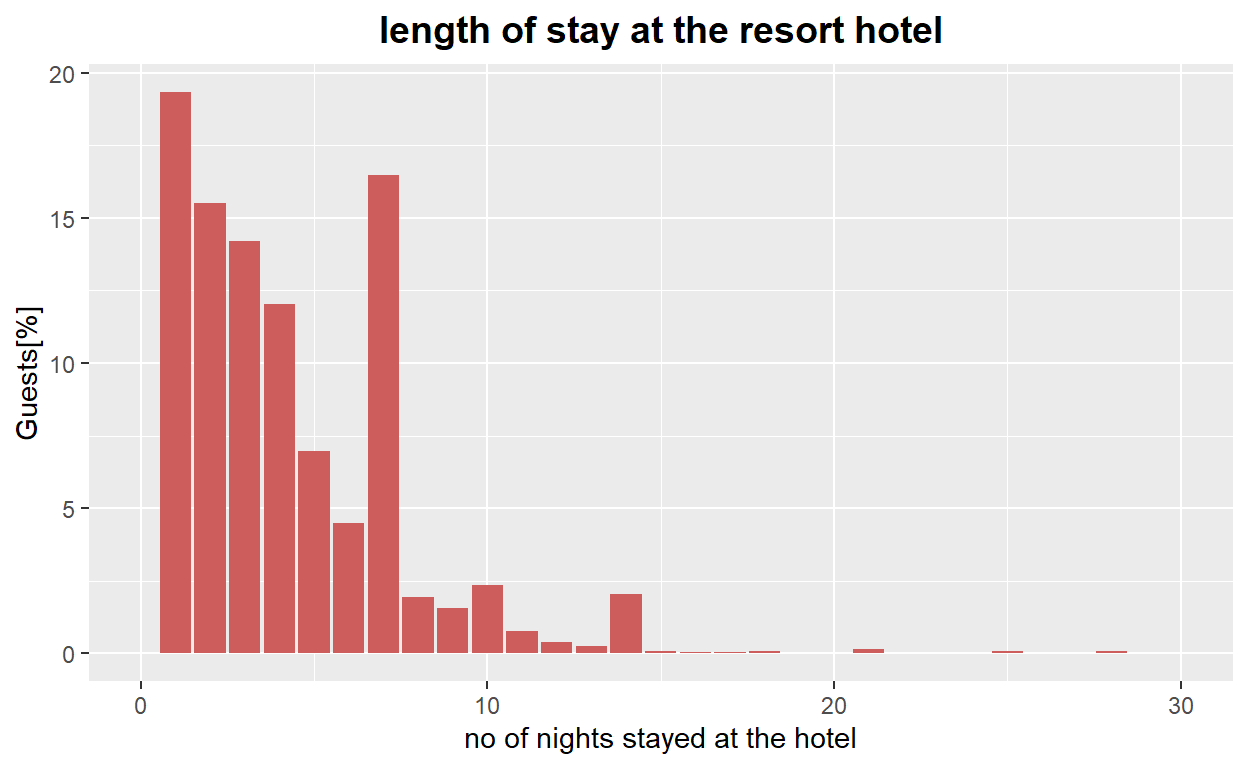
\includegraphics{AnkitFinalProject_files/figure-latex/unnamed-chunk-12-1.pdf}
Exploring the correlation between canceled hotel bookings and other
variables.

\begin{Shaded}
\begin{Highlighting}[]
\FunctionTok{cor}\NormalTok{(hotel\_bookings}\SpecialCharTok{$}\NormalTok{is\_canceled, hotel\_bookings}\SpecialCharTok{$}\NormalTok{previous\_cancellations)}
\end{Highlighting}
\end{Shaded}

\begin{verbatim}
## [1] 0.1101405
\end{verbatim}

\begin{Shaded}
\begin{Highlighting}[]
\FunctionTok{cor}\NormalTok{(hotel\_bookings}\SpecialCharTok{$}\NormalTok{is\_canceled, hotel\_bookings}\SpecialCharTok{$}\NormalTok{previous\_bookings\_not\_canceled)}
\end{Highlighting}
\end{Shaded}

\begin{verbatim}
## [1] -0.05735537
\end{verbatim}

\begin{Shaded}
\begin{Highlighting}[]
\FunctionTok{cor}\NormalTok{(hotel\_bookings}\SpecialCharTok{$}\NormalTok{is\_canceled, hotel\_bookings}\SpecialCharTok{$}\NormalTok{days\_in\_waiting\_list)}
\end{Highlighting}
\end{Shaded}

\begin{verbatim}
## [1] 0.05419315
\end{verbatim}

The correlations between canceled booking and above variables do not
appear to be strong. We will have to do a pairwise correlation for each
variable in the dataset.

Observing Lead Time by Customer Type in Hotels will provide insights on
the number of days elapsed between the booking date and arrival. Pricing
strategies can be made based on the availability of the rooms and the
lead time for each customer type.

\begin{Shaded}
\begin{Highlighting}[]
\NormalTok{hotel\_bookings  }\SpecialCharTok{\%\textgreater{}\%} \FunctionTok{select}\NormalTok{(customer\_type, lead\_time, hotel) }\SpecialCharTok{\%\textgreater{}\%} \FunctionTok{group\_by}\NormalTok{(customer\_type, hotel) }\SpecialCharTok{\%\textgreater{}\%} \FunctionTok{summarise}\NormalTok{(}\AttributeTok{mean =} \FunctionTok{round}\NormalTok{(}\FunctionTok{mean}\NormalTok{(lead\_time), }\DecValTok{2}\NormalTok{)) }\SpecialCharTok{\%\textgreater{}\%} \FunctionTok{ggplot}\NormalTok{(}\FunctionTok{aes}\NormalTok{(}\AttributeTok{x =}\NormalTok{ customer\_type, }\AttributeTok{y =}\NormalTok{ mean, }\AttributeTok{color =}\NormalTok{ hotel, }\AttributeTok{fill =}\NormalTok{ hotel)) }\SpecialCharTok{+} 
  \FunctionTok{geom\_point}\NormalTok{(}\AttributeTok{shape=}\DecValTok{21}\NormalTok{, }\AttributeTok{alpha=}\NormalTok{.}\DecValTok{55}\NormalTok{, }\AttributeTok{size=}\DecValTok{5}\NormalTok{) }\SpecialCharTok{+} 
  \FunctionTok{geom\_text}\NormalTok{(}\FunctionTok{aes}\NormalTok{(}\AttributeTok{label=}\NormalTok{mean,}\AttributeTok{vjust=}\SpecialCharTok{{-}}\FloatTok{0.3}\NormalTok{)) }\SpecialCharTok{+}
  \FunctionTok{labs}\NormalTok{(}\AttributeTok{title =} \StringTok{"Lead Time by Customer Type in Hotels"}\NormalTok{, }\AttributeTok{x =} \StringTok{"Customer Type"}\NormalTok{, }\AttributeTok{y =} \StringTok{"Lead time"}\NormalTok{) }\SpecialCharTok{+} \FunctionTok{theme\_classic}\NormalTok{() }\SpecialCharTok{+}
  \FunctionTok{theme}\NormalTok{(}\AttributeTok{plot.title =} \FunctionTok{element\_text}\NormalTok{(}\AttributeTok{face =} \StringTok{"bold"}\NormalTok{))}
\end{Highlighting}
\end{Shaded}

\begin{verbatim}
## `summarise()` has grouped output by 'customer_type'. You can override using the `.groups` argument.
\end{verbatim}

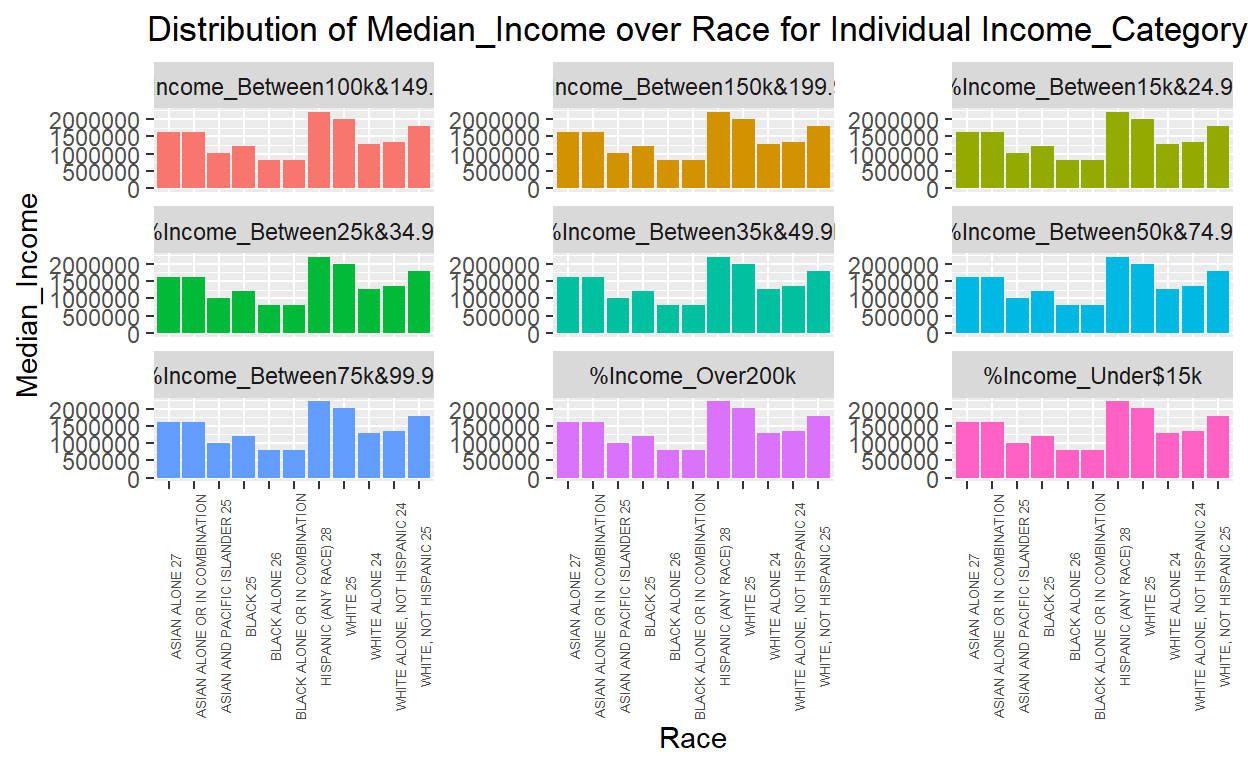
\includegraphics{AnkitFinalProject_files/figure-latex/unnamed-chunk-16-1.pdf}

Understanding the types of meal packages booked by customers. The type
of meal booked by customers can help the hotel management to derive paid
or complimentary meal packages to increase or generate a stream of
revenue.

\begin{Shaded}
\begin{Highlighting}[]
\NormalTok{(a }\OtherTok{\textless{}{-}}\NormalTok{ hotel\_bookings}\SpecialCharTok{\%\textgreater{}\%} \FunctionTok{select}\NormalTok{(meal, hotel) }\SpecialCharTok{\%\textgreater{}\%}  \FunctionTok{group\_by}\NormalTok{(meal, hotel) }\SpecialCharTok{\%\textgreater{}\%}  \FunctionTok{summarise}\NormalTok{(}\AttributeTok{freq =} \FunctionTok{n}\NormalTok{()))}
\end{Highlighting}
\end{Shaded}

\begin{verbatim}
## `summarise()` has grouped output by 'meal'. You can override using the `.groups` argument.
\end{verbatim}

\begin{verbatim}
## # A tibble: 9 x 3
## # Groups:   meal [5]
##   meal      hotel         freq
##   <chr>     <chr>        <int>
## 1 BB        City Hotel   62301
## 2 BB        Resort Hotel 30005
## 3 FB        City Hotel      44
## 4 FB        Resort Hotel   754
## 5 HB        City Hotel    6417
## 6 HB        Resort Hotel  8046
## 7 SC        City Hotel   10564
## 8 SC        Resort Hotel    86
## 9 Undefined Resort Hotel  1169
\end{verbatim}

\begin{Shaded}
\begin{Highlighting}[]
\FunctionTok{ggplot}\NormalTok{(a, }\FunctionTok{aes}\NormalTok{(}\AttributeTok{x=}\NormalTok{meal, }\AttributeTok{y=}\NormalTok{freq, }\AttributeTok{fill =}\NormalTok{ meal)) }\SpecialCharTok{+}
 \FunctionTok{geom\_bar}\NormalTok{(}\AttributeTok{stat=}\StringTok{"identity"}\NormalTok{) }\SpecialCharTok{+} \FunctionTok{facet\_wrap}\NormalTok{(}\SpecialCharTok{\textasciitilde{}}\NormalTok{hotel) }\SpecialCharTok{+}
\FunctionTok{geom\_text}\NormalTok{(}\FunctionTok{aes}\NormalTok{(}\AttributeTok{label=}\NormalTok{freq),}\AttributeTok{vjust=}\SpecialCharTok{{-}}\FloatTok{0.3}\NormalTok{)}\SpecialCharTok{+}
  \FunctionTok{labs}\NormalTok{(}\AttributeTok{title =} \StringTok{"Meals booked by Customers in Hotels"}\NormalTok{, }\AttributeTok{x =} \StringTok{"Meal"}\NormalTok{, }\AttributeTok{y =} \StringTok{"Number of meals"}\NormalTok{) }\SpecialCharTok{+}
 \FunctionTok{theme\_classic}\NormalTok{() }\SpecialCharTok{+}
 \FunctionTok{theme}\NormalTok{(}\AttributeTok{plot.title =} \FunctionTok{element\_text}\NormalTok{(}\AttributeTok{face =} \StringTok{"bold"}\NormalTok{))}
\end{Highlighting}
\end{Shaded}

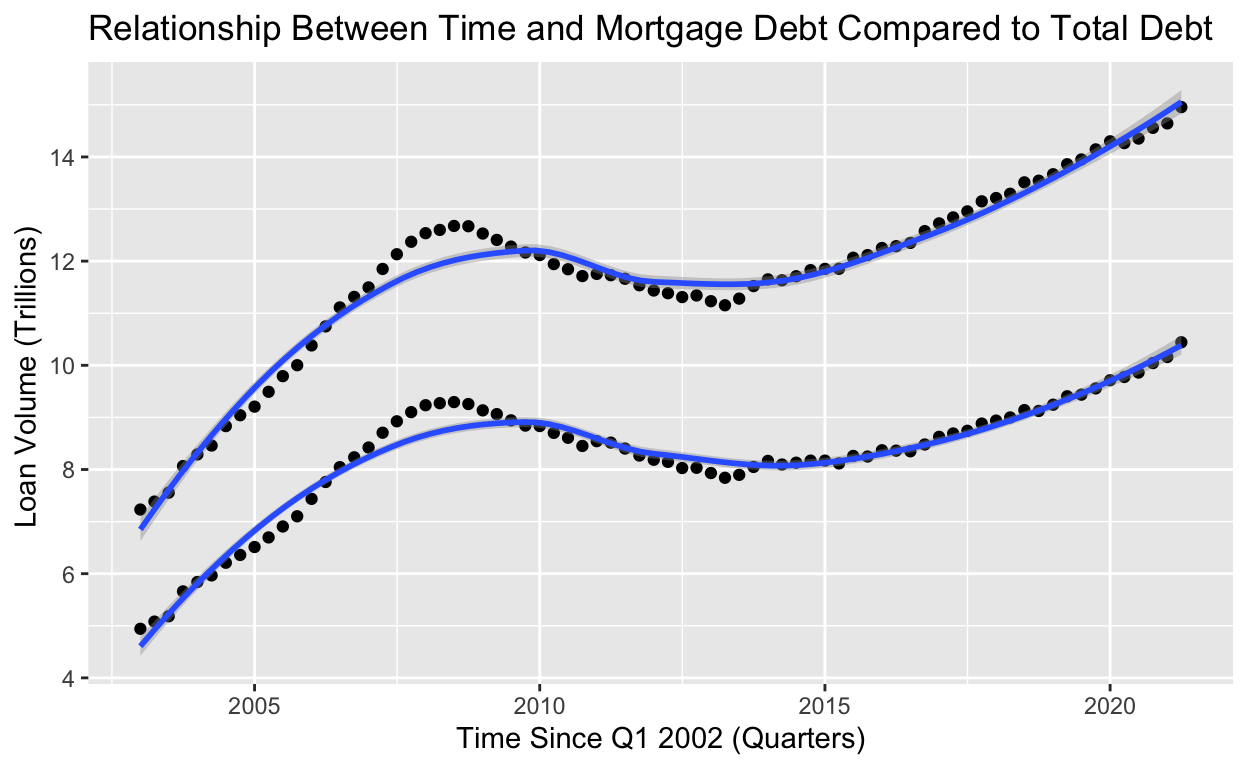
\includegraphics{AnkitFinalProject_files/figure-latex/unnamed-chunk-17-1.pdf}

What type of rooms are booked by customers? The type of rooms reserved
by customers shall provide cue to the hotels to curate their asset
management strategies.

\begin{Shaded}
\begin{Highlighting}[]
\NormalTok{hotel\_bookings }\SpecialCharTok{\%\textgreater{}\%} \FunctionTok{group\_by}\NormalTok{(reserved\_room\_type, hotel) }\SpecialCharTok{\%\textgreater{}\%} 
  \FunctionTok{select}\NormalTok{(reserved\_room\_type, hotel) }\SpecialCharTok{\%\textgreater{}\%} \FunctionTok{summarise}\NormalTok{(}\AttributeTok{freq =} \FunctionTok{n}\NormalTok{())}\SpecialCharTok{\%\textgreater{}\%} \FunctionTok{ggplot}\NormalTok{(}\FunctionTok{aes}\NormalTok{(}\AttributeTok{x =}\NormalTok{ reserved\_room\_type, }\AttributeTok{y=}\NormalTok{freq, }\AttributeTok{fill =}\NormalTok{ reserved\_room\_type)) }\SpecialCharTok{+}
  \FunctionTok{geom\_bar}\NormalTok{(}\AttributeTok{stat =} \StringTok{"identity"}\NormalTok{, }\AttributeTok{shape=}\DecValTok{21}\NormalTok{, }\AttributeTok{alpha=}\NormalTok{.}\DecValTok{55}\NormalTok{, }\AttributeTok{size=}\DecValTok{5}\NormalTok{) }\SpecialCharTok{+} \FunctionTok{facet\_wrap}\NormalTok{(}\SpecialCharTok{\textasciitilde{}}\NormalTok{hotel) }\SpecialCharTok{+} 
  \FunctionTok{geom\_text}\NormalTok{(}\FunctionTok{aes}\NormalTok{(}\AttributeTok{label=}\NormalTok{ freq),}\AttributeTok{vjust=} \SpecialCharTok{{-}}\FloatTok{0.3}\NormalTok{) }\SpecialCharTok{+}
  \FunctionTok{labs}\NormalTok{(}\AttributeTok{title =} \StringTok{"Type of rooms booked by Customers in Hotels"}\NormalTok{, }\AttributeTok{x =} \StringTok{"Type of Rooms reserved by Customers"}\NormalTok{, }\AttributeTok{y =} \StringTok{"Number of Rooms"}\NormalTok{) }\SpecialCharTok{+}
  \FunctionTok{theme\_gray}\NormalTok{() }\SpecialCharTok{+}
  \FunctionTok{theme}\NormalTok{( }\AttributeTok{plot.title =} \FunctionTok{element\_text}\NormalTok{(}\AttributeTok{face =} \StringTok{"bold"}\NormalTok{))}
\end{Highlighting}
\end{Shaded}

\begin{verbatim}
## `summarise()` has grouped output by 'reserved_room_type'. You can override using the `.groups` argument.
\end{verbatim}

\begin{verbatim}
## Warning: Ignoring unknown parameters: shape
\end{verbatim}

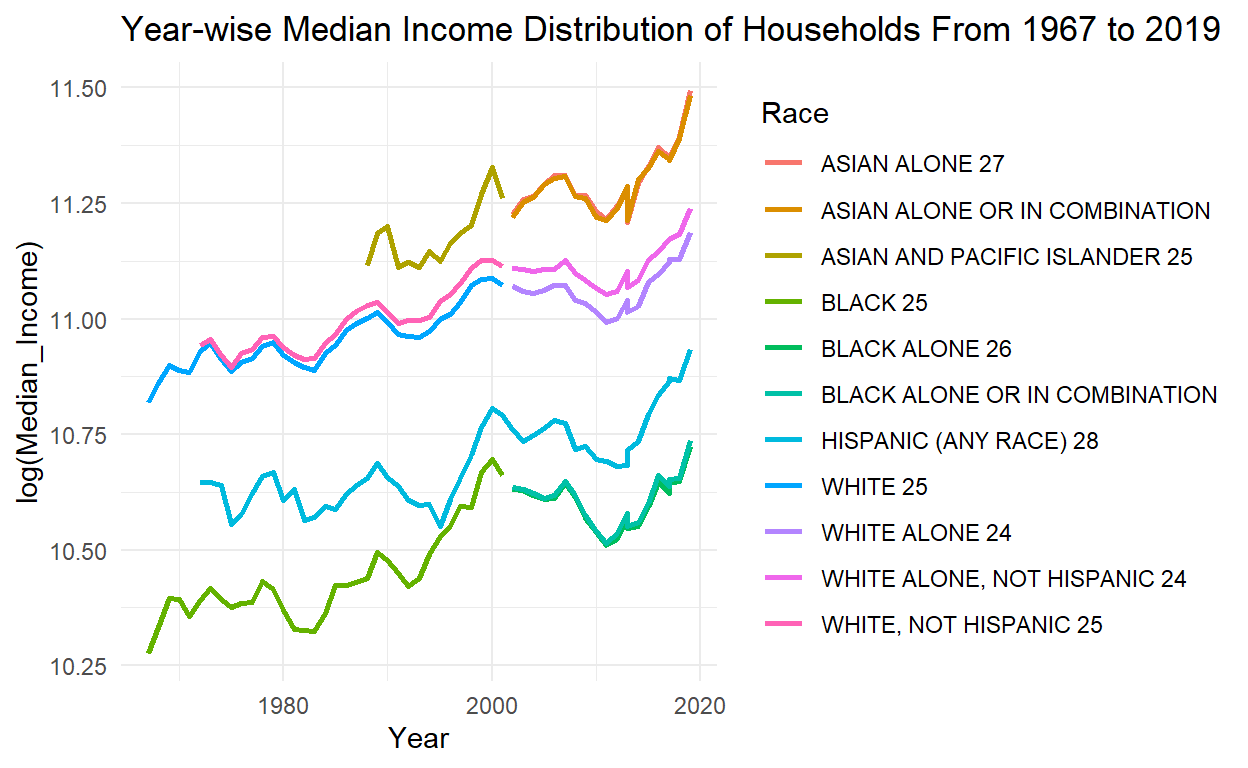
\includegraphics{AnkitFinalProject_files/figure-latex/unnamed-chunk-18-1.pdf}

The number of adults, children and babies visited the hotels will help
the hotel management to map the number and type of visitors with the
types of room that are availabe in the hotel.

\begin{Shaded}
\begin{Highlighting}[]
\NormalTok{hotel\_bookings }\SpecialCharTok{\%\textgreater{}\%} \FunctionTok{group\_by}\NormalTok{(hotel) }\SpecialCharTok{\%\textgreater{}\%} \FunctionTok{select}\NormalTok{(hotel, adults, children, babies)}\SpecialCharTok{\%\textgreater{}\%} \FunctionTok{summarize}\NormalTok{(}\AttributeTok{adults =} \FunctionTok{sum}\NormalTok{(adults), }\AttributeTok{children =} \FunctionTok{sum}\NormalTok{(children), }\AttributeTok{babies =} \FunctionTok{sum}\NormalTok{(babies))}
\end{Highlighting}
\end{Shaded}

\begin{verbatim}
## # A tibble: 2 x 4
##   hotel        adults children babies
##   <chr>         <dbl>    <dbl>  <dbl>
## 1 City Hotel   146829     7248    392
## 2 Resort Hotel  74798     5155    557
\end{verbatim}

How many customers were assigned a different room type than were
reserved by them? Could it be a reason for the cancellations?

\begin{Shaded}
\begin{Highlighting}[]
\NormalTok{hotel\_bookings }\SpecialCharTok{\%\textgreater{}\%} \FunctionTok{group\_by}\NormalTok{(hotel) }\SpecialCharTok{\%\textgreater{}\%} \FunctionTok{select}\NormalTok{(hotel, reserved\_room\_type, assigned\_room\_type) }\SpecialCharTok{\%\textgreater{}\%} \FunctionTok{mutate}\NormalTok{(}\AttributeTok{diff\_room\_assigned =} \FunctionTok{if\_else}\NormalTok{(assigned\_room\_type }\SpecialCharTok{!=}\NormalTok{ reserved\_room\_type, }\DecValTok{1}\NormalTok{, }\DecValTok{0}\NormalTok{)) }\SpecialCharTok{\%\textgreater{}\%} \FunctionTok{summarize}\NormalTok{(}\AttributeTok{diff\_room\_assigned =} \FunctionTok{sum}\NormalTok{(diff\_room\_assigned))}
\end{Highlighting}
\end{Shaded}

\begin{verbatim}
## # A tibble: 2 x 2
##   hotel        diff_room_assigned
##   <chr>                     <dbl>
## 1 City Hotel                 7192
## 2 Resort Hotel               7725
\end{verbatim}

\begin{Shaded}
\begin{Highlighting}[]
\NormalTok{hotel\_bookings }\SpecialCharTok{\%\textgreater{}\%} \FunctionTok{group\_by}\NormalTok{(hotel) }\SpecialCharTok{\%\textgreater{}\%} \FunctionTok{select}\NormalTok{(hotel, is\_canceled) }\SpecialCharTok{\%\textgreater{}\%} \FunctionTok{summarise}\NormalTok{(}\AttributeTok{is\_canceled =} \FunctionTok{sum}\NormalTok{(is\_canceled)) }
\end{Highlighting}
\end{Shaded}

\begin{verbatim}
## # A tibble: 2 x 2
##   hotel        is_canceled
##   <chr>              <dbl>
## 1 City Hotel         33098
## 2 Resort Hotel       11122
\end{verbatim}

Observing cancellation by customer type

\begin{Shaded}
\begin{Highlighting}[]
\NormalTok{hotel\_bookings }\SpecialCharTok{\%\textgreater{}\%} \FunctionTok{group\_by}\NormalTok{(hotel, customer\_type) }\SpecialCharTok{\%\textgreater{}\%} \FunctionTok{select}\NormalTok{(hotel, is\_canceled, customer\_type) }\SpecialCharTok{\%\textgreater{}\%} \FunctionTok{summarise}\NormalTok{(}\AttributeTok{is\_canceled =} \FunctionTok{sum}\NormalTok{(is\_canceled))}\SpecialCharTok{\%\textgreater{}\%} \FunctionTok{ggplot}\NormalTok{(}\FunctionTok{aes}\NormalTok{(}\AttributeTok{x =}\NormalTok{ customer\_type, }\AttributeTok{y =}\NormalTok{ is\_canceled)) }\SpecialCharTok{+}
  \FunctionTok{geom\_bar}\NormalTok{(}\AttributeTok{position =} \StringTok{"dodge"}\NormalTok{, }\AttributeTok{stat =} \StringTok{"identity"}\NormalTok{, }\AttributeTok{fill =} \StringTok{"chartreuse"}\NormalTok{) }\SpecialCharTok{+}
  \FunctionTok{theme\_classic}\NormalTok{() }\SpecialCharTok{+}
  \FunctionTok{labs}\NormalTok{(}\AttributeTok{title =} \StringTok{"Number of Cancellations by type of Customers in Hotels"}\NormalTok{, }\AttributeTok{x =} \StringTok{"Type of Customer"}\NormalTok{, }\AttributeTok{y =} \StringTok{"Number of Customers"}\NormalTok{) }\SpecialCharTok{+}
  \FunctionTok{theme}\NormalTok{(}\AttributeTok{plot.title =} \FunctionTok{element\_text}\NormalTok{(}\AttributeTok{face =} \StringTok{"bold"}\NormalTok{))}
\end{Highlighting}
\end{Shaded}

\begin{verbatim}
## `summarise()` has grouped output by 'hotel'. You can override using the `.groups` argument.
\end{verbatim}

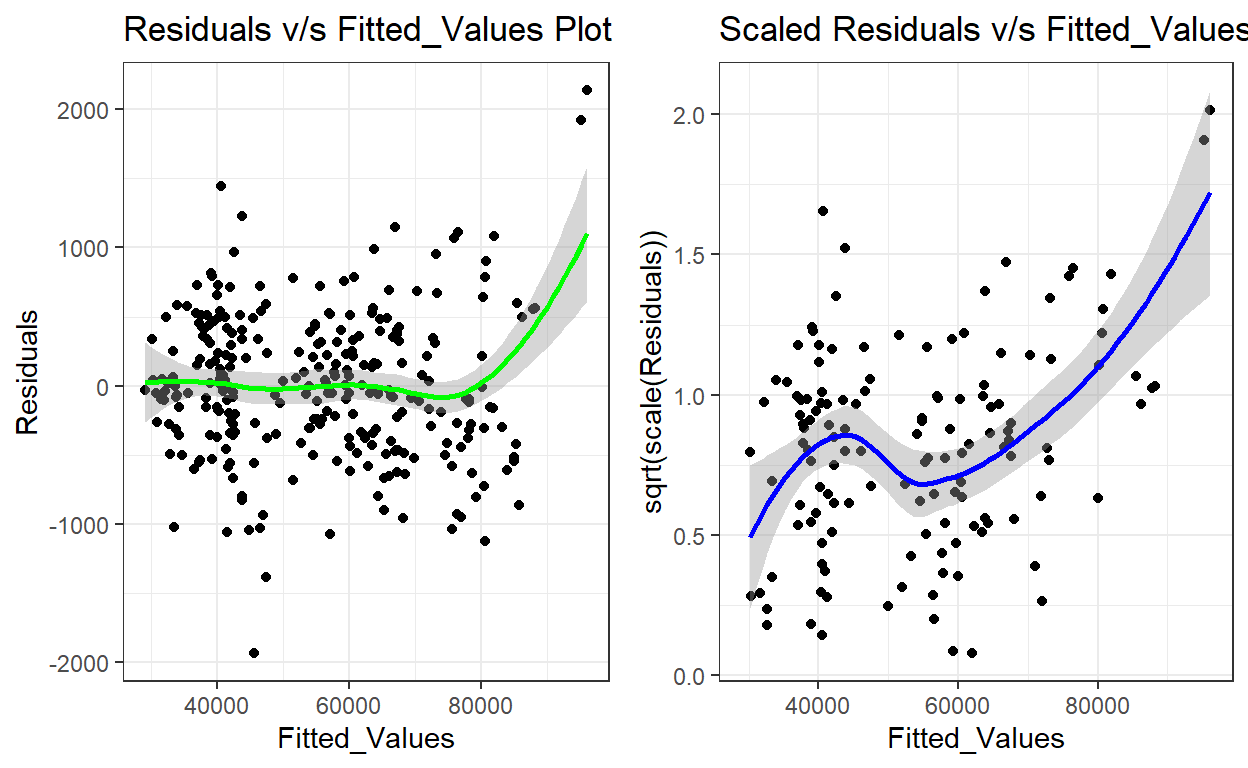
\includegraphics{AnkitFinalProject_files/figure-latex/unnamed-chunk-22-1.pdf}

The footfall of visitors in each month will help the hotel management to
develop strategies that generate demand in lean seasons.

\begin{Shaded}
\begin{Highlighting}[]
\NormalTok{hotel\_bookings }\SpecialCharTok{\%\textgreater{}\%}
  \FunctionTok{select}\NormalTok{(hotel, arrival\_date\_month) }\SpecialCharTok{\%\textgreater{}\%} \FunctionTok{group\_by}\NormalTok{(hotel, arrival\_date\_month) }\SpecialCharTok{\%\textgreater{}\%} 
    \FunctionTok{tally}\NormalTok{(}\AttributeTok{name =} \StringTok{"freq"}\NormalTok{) }\SpecialCharTok{\%\textgreater{}\%}
  \FunctionTok{ggplot}\NormalTok{(}\FunctionTok{aes}\NormalTok{(}\AttributeTok{x =}\NormalTok{ freq, }\AttributeTok{y =}\NormalTok{ arrival\_date\_month)) }\SpecialCharTok{+}
  \FunctionTok{geom\_bar}\NormalTok{(}\AttributeTok{position =} \StringTok{"dodge"}\NormalTok{, }\AttributeTok{stat =} \StringTok{"identity"}\NormalTok{, }\AttributeTok{fill =} \StringTok{"chartreuse"}\NormalTok{) }\SpecialCharTok{+}
  \FunctionTok{theme\_classic}\NormalTok{() }\SpecialCharTok{+}
  \FunctionTok{labs}\NormalTok{(}\AttributeTok{title =} \StringTok{"Number of arrivals in each month"}\NormalTok{, }\AttributeTok{x =} \StringTok{"Number of reservations"}\NormalTok{,}
       \AttributeTok{y =} \StringTok{"Month"}\NormalTok{) }\SpecialCharTok{+}
  \FunctionTok{theme}\NormalTok{(}\AttributeTok{plot.title =} \FunctionTok{element\_text}\NormalTok{(}\AttributeTok{face =} \StringTok{"bold"}\NormalTok{))}
\end{Highlighting}
\end{Shaded}

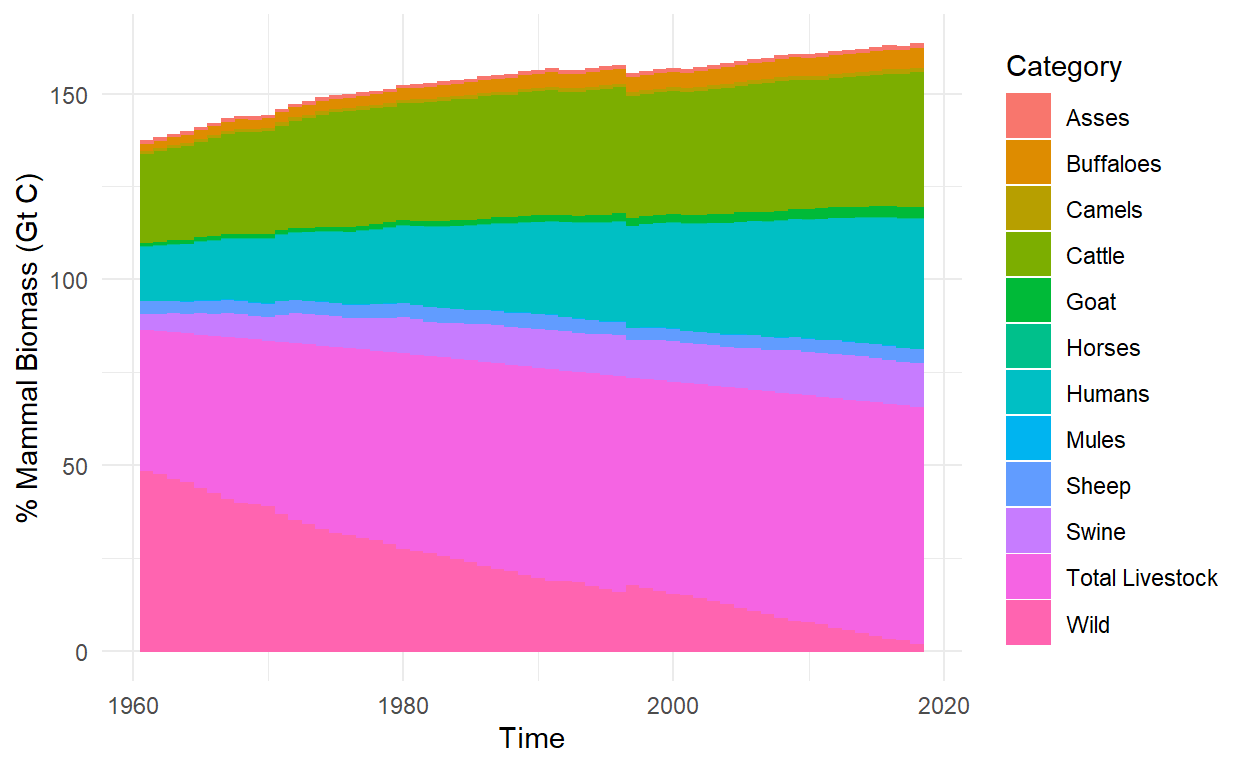
\includegraphics{AnkitFinalProject_files/figure-latex/unnamed-chunk-23-1.pdf}

Segregating hotel data set into city hotels and resort hotels will help
us exploring the intricacies and anomalies involved in the data with
respect to city and resort hotels per se.

\begin{Shaded}
\begin{Highlighting}[]
\NormalTok{city\_hotel }\OtherTok{\textless{}{-}}\NormalTok{ hotel\_bookings }\SpecialCharTok{\%\textgreater{}\%} \FunctionTok{filter}\NormalTok{(hotel\_bookings}\SpecialCharTok{$}\NormalTok{hotel }\SpecialCharTok{==} \StringTok{"City Hotel"}\NormalTok{)}

\NormalTok{resort\_hotel }\OtherTok{\textless{}{-}}\NormalTok{ hotel\_bookings }\SpecialCharTok{\%\textgreater{}\%} \FunctionTok{filter}\NormalTok{(hotel\_bookings}\SpecialCharTok{$}\NormalTok{hotel }\SpecialCharTok{==} \StringTok{"Resort Hotel"}\NormalTok{)}
\end{Highlighting}
\end{Shaded}

Exploring City Hotels and Resort Hotels further.

Frequency table of the market segment in city hotels.

\begin{Shaded}
\begin{Highlighting}[]
\NormalTok{n\_cityHotel\_mktSegment }\OtherTok{\textless{}{-}}\NormalTok{ city\_hotel }\SpecialCharTok{\%\textgreater{}\%}
  \FunctionTok{group\_by}\NormalTok{(market\_segment) }\SpecialCharTok{\%\textgreater{}\%} \FunctionTok{count}\NormalTok{(customer\_type)}

\NormalTok{n\_cityHotel\_mktSegment}
\end{Highlighting}
\end{Shaded}

\begin{verbatim}
## # A tibble: 26 x 3
## # Groups:   market_segment [7]
##    market_segment customer_type       n
##    <chr>          <chr>           <int>
##  1 Aviation       Group               2
##  2 Aviation       Transient         218
##  3 Aviation       Transient-Party    17
##  4 Complementary  Contract            1
##  5 Complementary  Group               5
##  6 Complementary  Transient         516
##  7 Complementary  Transient-Party    20
##  8 Corporate      Group              16
##  9 Corporate      Transient        1955
## 10 Corporate      Transient-Party  1015
## # ... with 16 more rows
\end{verbatim}

Observing Number of Customers by the type of customers and market
segment in city hotels.

\begin{Shaded}
\begin{Highlighting}[]
\NormalTok{n\_cityHotel\_mktSegment }\SpecialCharTok{\%\textgreater{}\%} 
\FunctionTok{ggplot}\NormalTok{(}\FunctionTok{aes}\NormalTok{(}\AttributeTok{x =}\NormalTok{ market\_segment, }\AttributeTok{y =}\NormalTok{ n, }\AttributeTok{fill =}\NormalTok{ customer\_type)) }\SpecialCharTok{+}
  \FunctionTok{geom\_bar}\NormalTok{(}\AttributeTok{position =} \StringTok{"dodge"}\NormalTok{, }\AttributeTok{stat =} \StringTok{"identity"}\NormalTok{) }\SpecialCharTok{+}
  \FunctionTok{theme\_classic}\NormalTok{() }\SpecialCharTok{+}
  \FunctionTok{labs}\NormalTok{(}\AttributeTok{title =} \StringTok{"Number of Customers in NYC City Hotels by market segment"}\NormalTok{, }\AttributeTok{x =} \StringTok{"Market Segment"}\NormalTok{, }\AttributeTok{y =} \StringTok{"Number of Customers"}\NormalTok{) }\SpecialCharTok{+}
  \FunctionTok{theme}\NormalTok{(}\AttributeTok{plot.title =} \FunctionTok{element\_text}\NormalTok{(}\AttributeTok{face =} \StringTok{"bold"}\NormalTok{))}
\end{Highlighting}
\end{Shaded}

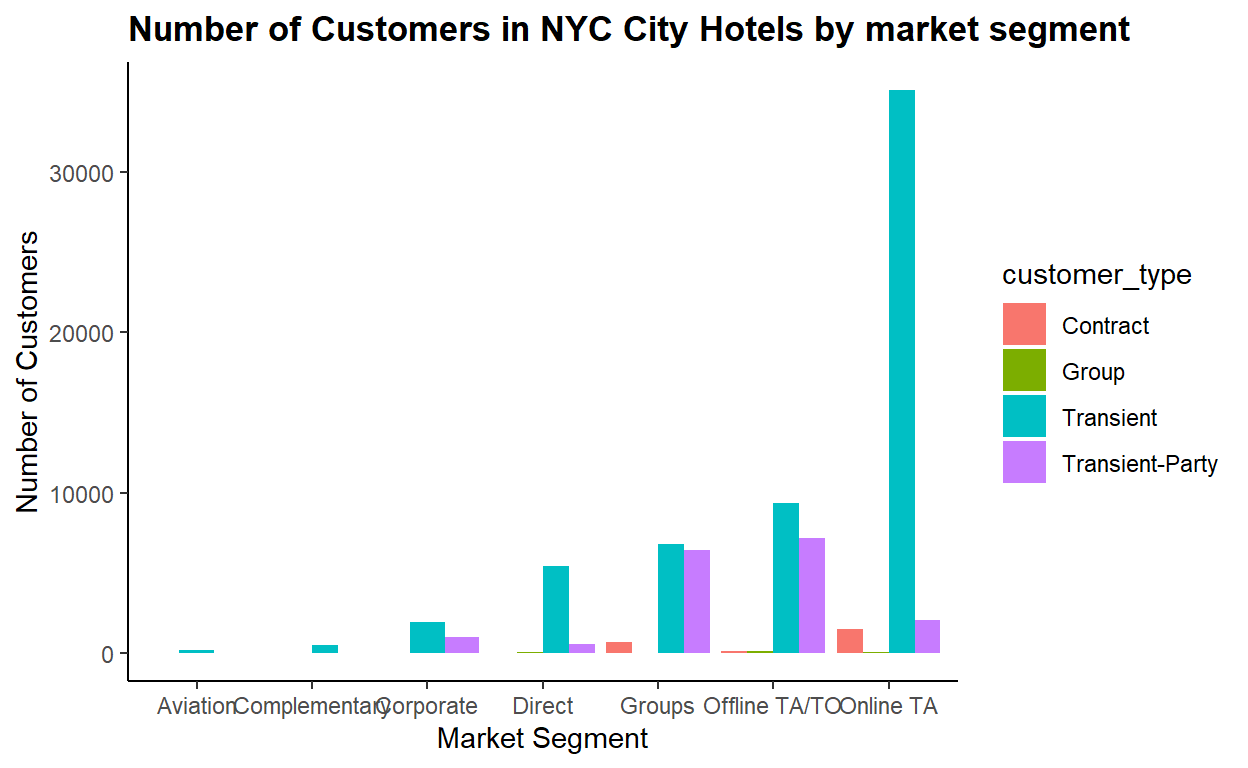
\includegraphics{AnkitFinalProject_files/figure-latex/unnamed-chunk-26-1.pdf}

Frequency table of the market segment in resort hotels.

\begin{Shaded}
\begin{Highlighting}[]
\NormalTok{n\_resortHotel\_mktSegment }\OtherTok{\textless{}{-}}\NormalTok{ resort\_hotel }\SpecialCharTok{\%\textgreater{}\%}
  \FunctionTok{group\_by}\NormalTok{(market\_segment) }\SpecialCharTok{\%\textgreater{}\%} \FunctionTok{count}\NormalTok{(customer\_type)}

\NormalTok{n\_resortHotel\_mktSegment}
\end{Highlighting}
\end{Shaded}

\begin{verbatim}
## # A tibble: 24 x 3
## # Groups:   market_segment [6]
##    market_segment customer_type       n
##    <chr>          <chr>           <int>
##  1 Complementary  Contract            1
##  2 Complementary  Group               1
##  3 Complementary  Transient         187
##  4 Complementary  Transient-Party    12
##  5 Corporate      Contract           22
##  6 Corporate      Group              13
##  7 Corporate      Transient        1621
##  8 Corporate      Transient-Party   653
##  9 Direct         Contract           12
## 10 Direct         Group              82
## # ... with 14 more rows
\end{verbatim}

Observing Number of Customers by the type of customers and market
segment in resort hotels.

\begin{Shaded}
\begin{Highlighting}[]
\NormalTok{n\_resortHotel\_mktSegment }\SpecialCharTok{\%\textgreater{}\%} 
\FunctionTok{ggplot}\NormalTok{(}\FunctionTok{aes}\NormalTok{(}\AttributeTok{x =}\NormalTok{ market\_segment, }\AttributeTok{y =}\NormalTok{ n, }\AttributeTok{fill =}\NormalTok{ customer\_type)) }\SpecialCharTok{+}
  \FunctionTok{geom\_bar}\NormalTok{(}\AttributeTok{position =} \StringTok{"dodge"}\NormalTok{, }\AttributeTok{stat =} \StringTok{"identity"}\NormalTok{) }\SpecialCharTok{+}
  \FunctionTok{theme\_classic}\NormalTok{() }\SpecialCharTok{+}
  \FunctionTok{labs}\NormalTok{(}\AttributeTok{title =} \StringTok{"Number of Customers in Resort Hotels by market segment"}\NormalTok{, }\AttributeTok{x =} \StringTok{"Market Segment"}\NormalTok{, }\AttributeTok{y =} \StringTok{"Number of Customers"}\NormalTok{) }\SpecialCharTok{+}
  \FunctionTok{theme}\NormalTok{(}\AttributeTok{plot.title =} \FunctionTok{element\_text}\NormalTok{(}\AttributeTok{face =} \StringTok{"bold"}\NormalTok{))}
\end{Highlighting}
\end{Shaded}

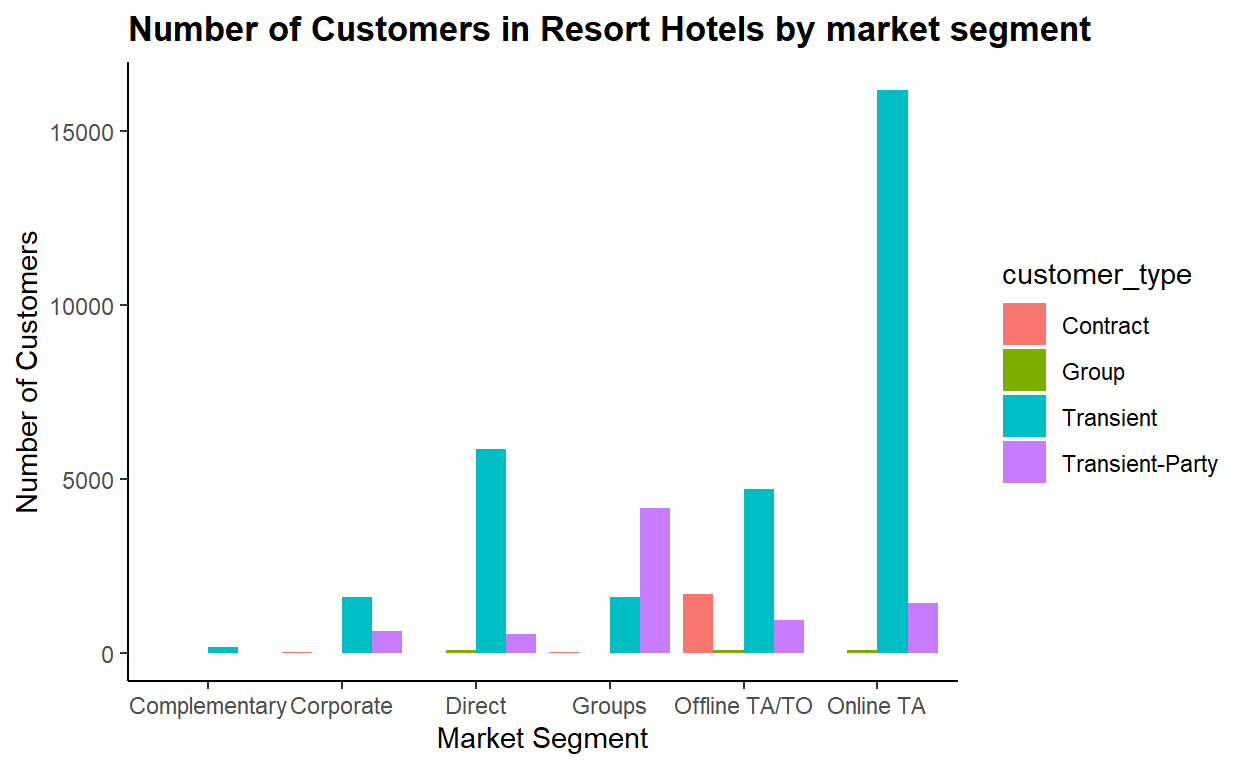
\includegraphics{AnkitFinalProject_files/figure-latex/unnamed-chunk-28-1.pdf}

<!--radix_placeholder_site_after_body-->
<!--/radix_placeholder_site_after_body-->

<!--radix_placeholder_navigation_after_body-->
<div class="distill-site-nav distill-site-footer">
<!-- DACSS wordmark -->
<div class="footer-center"><a href="https://www.umass.edu/sbs/dacss">
  <img src="images/white-dacss-wordmark.png" 
  alt="UMass Amherst DACSS" width ="30%" id="dacss-footer"/></a>
</div>
<!-- Social media icons -->
<div class="container">
  <div class="social-media-icons">
    <a href="https://twitter.com/UMassDACSS" target="_blank" title="Twitter" class="footer fa fa-twitter"></a>
    <a href="https://bit.ly/3cMIlIK" target="_blank" title="Facebook" class="footer fa fa-facebook"></a>
    <a href="https://bit.ly/2PymwUp" target="_blank" title="LinkedIn" class="footer fa fa-linkedin"></a>
    <a href="https://www.instagram.com/umassdacss/?hl=en" target="_blank" title="Instagram" class="footer fa fa-instagram"></a>
    <a class="fa fa-placeholder"></a>
  </div>
</div>
</div>
<!--/radix_placeholder_navigation_after_body-->


\end{document}
